\documentclass[a4paper, twoside]{report}

%% Language and font encodings
\usepackage[english]{babel}
\usepackage[utf8]{inputenc}
\usepackage[T1]{fontenc}
\usepackage{booktabs}
\usepackage{placeins}
\usepackage{tabularx}
\usepackage{longtable}
\setcounter{secnumdepth}{3}
\usepackage{array}
\usepackage{subcaption}
\usepackage[table]{xcolor}
\usepackage{multirow}

\newcolumntype{M}[1]{>{\centering\arraybackslash}m{#1}}

%% Sets page size and margins
\usepackage[a4paper,top=3cm,bottom=2cm,left=3cm,right=3cm,marginparwidth=1.75cm]{geometry}

%% Useful packages
\usepackage{amsmath}
\usepackage{amssymb}
\usepackage{graphicx}
\usepackage[colorinlistoftodos]{todonotes}
\usepackage[colorlinks=true, allcolors=blue]{hyperref}
\usepackage{fancyhdr}

\usepackage{parskip}

%% Diagrams
\usepackage{tikz}
\usetikzlibrary{shapes.geometric, arrows.meta, positioning, calc, fit,
                backgrounds, decorations.pathreplacing, angles, quotes, patterns}

\begin{document}
\begin{titlepage}
\thispagestyle{empty}

\newcommand{\HRule}{\noindent\rule{\textwidth}{0.5mm}}
\newcommand{\ReportTitle}{A Guided, Self-Evaluating Stereo Calibration Procedure}

%----------------------------------------------------------------------------------------
%	LOGO SECTION
%----------------------------------------------------------------------------------------

\noindent
\begin{minipage}[t]{0.15\textwidth}
    
\includegraphics[width=2cm]{title/Logo_APSCO.png}
\end{minipage}%
\hfill
\begin{minipage}[t]{0.8\textwidth}
    \raggedleft
    {\Huge \textbf{APSCO}}
\end{minipage}
\HRule

%----------------------------------------------------------------------------------------
%	HEADING SECTIONS
%----------------------------------------------------------------------------------------

\begin{center}
\vspace{0.5cm}
{\textbf{\LARGE LINKU Project}\par}
\vspace{0.5cm}
{\textsc{\Large Camera System Working Document}\par}
\vspace{1cm}
\vspace{0.25cm}
{\textsc{\Large "Calibration Method and Tool Design"}\par}
\vspace{0.5cm}

%----------------------------------------------------------------------------------------
%	DATE SECTION
%----------------------------------------------------------------------------------------

{\Large \today\par}
\vspace{0.5cm}
\nointerlineskip

%----------------------------------------------------------------------------------------
%   TITLE SECTION
%----------------------------------------------------------------------------------------

\HRule
\vspace{0.20cm}
{\huge \bfseries \ReportTitle\par}
\vspace{0.20cm}
\HRule
\end{center}

%----------------------------------------------------------------------------------------
%	DOCUMENT INFORMATION SECTION
%----------------------------------------------------------------------------------------

\vspace{0.2cm}
\begingroup
\large
\setlength{\parindent}{0pt}
\raggedright

\textbf{Prepared by:}\par
\vspace{0.2cm}

\textsuperscript{1} Pontificia Universidad Catolica del Peru (PUCP)\par
\vspace{0.1cm}


\textbf{Author(s):} Jose Sifuentes\textsuperscript{1}\par
\vspace{0.2cm}

\textbf{Status:} Literature review complete, tool implemented, remedy not yet confirmed on hardware\par
\vspace{0.5cm}

\textbf{Issue:} 1\par
\textbf{Revision:} 0
\endgroup

%----------------------------------------------------------------------------------------
%	BOTTOM LOGOS
%----------------------------------------------------------------------------------------

\vfill
\begin{center}
    
\includegraphics[width=1\textwidth]{title/Logo_LINKUTEAM.png}
\end{center}

\end{titlepage}


\begin{abstract}
The LINKU stereo pair has been calibrated 23 times without reaching acceptable quality. This document asks why, and what the published literature says a calibration procedure should look like, and converts the answer into a specification for a replacement tool.

Three findings drive the design. First, the quantity the project currently uses to judge a calibration, the root-mean-square reprojection error, is a \emph{training} residual and can be made arbitrarily small by a badly chosen set of images; the literature is unanimous that it is not a measure of calibration quality. Second, calibration accuracy is dominated by the choice of target poses, and specific pose configurations are mathematically degenerate: with the board parallel to the sensor in every view the focal length is simply not recoverable, no matter how many images are taken. Third, every modern system that solves this problem does the same thing: it estimates the covariance of the calibration parameters while the session runs, uses it both to tell the operator where to put the board next and to decide when the calibration has converged.

Chapter \ref{chap:failure} analyses what can invalidate a calibration in this specific setup, including the two questions that prompted this document: whether capture resolution must match, and whether moving the focus or the aperture ring breaks the result. Chapter \ref{chap:literature} reviews the method, from Zhang's formulation to the four guided-calibration systems that implement live pose suggestion. Chapter \ref{chap:quality} sets out how to measure calibration quality honestly. Chapter \ref{chap:design} specifies the proposed tool: continuous capture with automatic frame gating, a live per-frame verdict, and a convergence bar driven by parameter uncertainty rather than by a frame count. Chapter \ref{chap:plan} gives a staged implementation plan against the project's existing code.

No part of the proposed tool has been implemented yet. The design is traceable to the eleven papers archived in \texttt{Sources/}; the wider set consulted but not cited is kept in the research folder \texttt{Investigacion/\allowbreak Calibracion\_Estereo}.
\end{abstract}

\tableofcontents
\listoffigures
\listoftables

\chapter*{Introduction}
\addcontentsline{toc}{chapter}{Introduction}

\section*{The problem this document addresses}

The LINKU camera system reconstructs the geometry of a thin tether from stereo imagery. Every number that pipeline produces is scaled and shaped by the calibration: the intrinsic parameters of each camera and the rigid transform between them. The project's calibration directory contains 23 attempts, none of which reached the quality target, and the current procedure offers no way to tell, during a session, whether the images being collected are improving the result or wasting time.

That is not an unusual situation. The literature is explicit that calibration is hard to perform reliably without expert intuition, and that even researchers working in the field struggle to say what makes a good calibration image \cite{rojtberg2018pose}. What is unusual is to keep repeating the procedure without changing it. This document changes it.

\section*{The two questions that started this}

The immediate trigger was a pair of practical questions from the operator, both of which turn out to be well founded and both of which are answered in Chapter \ref{chap:failure}:

\begin{itemize}
    \item \textbf{Must every image be captured at the same resolution, and is the calibration invalid if the capture resolution differs from the calibration resolution?} Yes to both, and the reason is more subtle than a simple rescaling, because changing sensor mode on this camera mixes binning with cropping.
    \item \textbf{The lens has an adjustable aperture and a manual focus ring. If either moves, does the calibration break?} Focus, yes, badly. Aperture, much less, but not innocently.
\end{itemize}

\section*{What is proposed}

A calibration session should not be a fixed ritual of ``take 25 photos and hope''. It should be a closed loop that measures its own progress. The proposal, specified in Chapter \ref{chap:design}, has three parts:

\begin{enumerate}
    \item \textbf{Continuous capture with automatic gating.} The operator moves the board; the tool decides which frames to keep. Frames are rejected for blur, for incomplete detection, and for carrying no new information.
    \item \textbf{A live verdict per frame.} Accepted, rejected and why, shown immediately, so the operator learns what the tool wants rather than guessing.
    \item \textbf{A convergence indicator driven by parameter uncertainty.} Not a count of images, but an estimate of how far the current solution is from being well determined, with an explicit stopping criterion.
\end{enumerate}

All three are established techniques, not inventions of this document. Chapter \ref{chap:literature} identifies the four systems that implement them and what each contributes.

\section*{Scope}

This document covers the calibration \emph{method and tool}. It does not cover the illumination of the calibration session, which is specified in the companion deliverable \cite{linku_darkroom_illumination}, nor the reconstruction pipeline that consumes the calibration. The target hardware is the IMX477 stereo pair with the 8~mm Arducam C1508ZM04 lens currently fitted, as recorded in the camera system report.

\section*{On sources}

Eleven papers are cited and archived in \texttt{Sources/}. The broader set of material consulted but not cited is in \texttt{Documentation/Investigacion/Calibracion\_Estereo/}. Where a claim rests on the project's own code or data rather than on the literature, the text says so.

\chapter{What Invalidates a Calibration}
\label{chap:failure}

Before proposing a better tool it is worth being precise about what a calibration actually estimates, and about which physical changes destroy it. This chapter answers the two operator questions that prompted the document, then collects the other failure modes that bear on the 23 unsuccessful attempts.

\section{What is being estimated, and from which images}

A common misconception is that intrinsic and extrinsic parameters come from different photographs. They do not. Both are recovered from the \emph{same} set of images, in a single joint optimisation \cite{zhang2000flexible}. What differs is what each group describes.

\begin{table}[!ht]
\centering
\small
\caption[Parameters recovered by a stereo calibration]{What a stereo calibration estimates. The per-view board poses are nuisance parameters: they are solved for because they must be, then discarded.}
\label{tab:params}
\begin{tabularx}{\textwidth}{p{0.17\textwidth} p{0.25\textwidth} X}
\toprule
\textbf{Group} & \textbf{Parameters} & \textbf{Scope} \\
\midrule
Intrinsics & $f_x, f_y, c_x, c_y$ and the distortion coefficients $k_1, k_2, k_3, p_1, p_2$ & One set per camera, shared by every image that camera took \\
Stereo extrinsics & $R, T$ between the two cameras & One single transform for the whole rig, from the frames where both cameras see the board \\
Board poses & $R_j, T_j$ per view & One per image; discarded after the fit \\
\bottomrule
\end{tabularx}
\end{table}

Rotating and tilting the board is therefore not a step that serves the extrinsics. It is what makes the \emph{intrinsics} observable at all, for a reason made precise in Section \ref{sec:degeneracy}.

\section{Resolution: it must match, and rescaling is not always possible}
\label{sec:resolution}

The intrinsics are expressed in pixels. Writing $p$ for the pixel pitch and $f$ for the focal length in millimetres,

\begin{equation}
f_x = \frac{f}{p_x}, \qquad f_y = \frac{f}{p_y} ,
\label{eq:fx}
\end{equation}

so any change in the effective pixel pitch changes $f_x$ and $f_y$ directly. The distortion coefficients are defined on normalised image coordinates and are, to first order, resolution-independent; the four pinhole parameters are not.

The temptation is to assume a calibration can always be rescaled by the resolution ratio. That holds only when the change is a pure scaling of the same field of view. Sensor modes mix two different operations:

\begin{itemize}
    \item \textbf{Binning or downscaling} keeps the field of view and enlarges the effective pixel. Then $f_x, f_y, c_x, c_y$ all divide by the same factor $s$, and the calibration can be rescaled exactly.
    \item \textbf{Cropping} keeps the pixel pitch and discards part of the field. Then $f_x, f_y$ are unchanged while $c_x, c_y$ shift by the crop offset. A naive rescale by the resolution ratio is simply wrong.
\end{itemize}

Table \ref{tab:modes} applies this to the modes the IMX477 actually offers \cite{raspberrypi_camera_docs_placeholder}. Two of them are not rescalings at all.

\begin{table}[!ht]
\centering
\small
\caption[IMX477 modes and whether a calibration can be rescaled between them]{Scale factors from the full 4056$\times$3040 readout to each mode. When the horizontal and vertical factors differ, the mode involves a crop and the calibration cannot be transferred by a single ratio. Modes as published by Raspberry Pi; factors computed for this document.}
\label{tab:modes}
\begin{tabularx}{\textwidth}{l c c X}
\toprule
\textbf{Mode} & \textbf{$s_x$} & \textbf{$s_y$} & \textbf{Interpretation} \\
\midrule
4056$\times$3040 & 1.000 & 1.000 & Full readout. The reference, and what this project captures at. \\
2028$\times$1520 & 2.000 & 2.000 & Pure 2$\times$2 binning, same field. Rescalable exactly. \\
2028$\times$1080 & 2.000 & 2.815 & Binned \emph{and} cropped: about 29\% of the vertical field is discarded. Not rescalable. \\
1332$\times$990  & 3.045 & 3.071 & Scaled and slightly cropped. Not rescalable. \\
1920$\times$1440 & 2.1125 & 2.1111 & The project's preview resolution. Close to a pure rescale, but the 0.066\% mismatch in aspect ratio shows a residual crop or anisotropic scale. \\
\bottomrule
\end{tabularx}
\end{table}

\paragraph{Answer to the operator's question.} Yes, every calibration image must be captured at the same resolution \emph{and the same sensor mode} as the images the calibration will be applied to. In principle a pure-binning change can be compensated analytically, but the project's own code already notes that without an explicit \texttt{-{}-mode} argument libcamera may silently choose a mode and then scale or crop, which makes the transfer untrustworthy in practice. The existing code is correct on this point: it forces calibration captures to the full \texttt{capture\_resolution} and passes \texttt{-{}-mode} explicitly. That behaviour must be preserved by any new tool.

\section{Focus: this one breaks the calibration}

On a manual C-mount lens such as the fitted C1508ZM04, focusing physically displaces the optical group relative to the sensor. That changes the effective focal length, and by Equation \ref{eq:fx} it changes $f_x$ and $f_y$ in direct proportion. The effect is known as focus breathing and it is not small on short-focal-length lenses.

The consequence for this project is a \emph{scale error on every reconstructed distance}. A relative error $\epsilon$ in the focal length propagates to a relative error $\epsilon$ in the triangulated depth, so a 1\% focus drift becomes a 10~mm bias on a 1~m measurement. That is a systematic bias, not noise: averaging more frames does not remove it.

\textbf{If the focus ring moves after calibration, the calibration is invalid.} This is the failure mode to guard against, and it is aggravated here because the experiment deliberately moves the rig by hand.

\section{Aperture: milder, but not free}

Changing the aperture is geometrically much more benign:

\begin{itemize}
    \item The focal length is nominally unchanged, so $f_x$ and $f_y$ are preserved.
    \item The principal point can shift slightly, because stopping down changes which cone of rays reaches each pixel and real irises are not perfectly centred on the optical axis.
    \item The measured distortion changes slightly, for the same reason: different apertures sample different zones of the lens.
    \item Depth of field, diffraction and aberrations change substantially. This is the dominant practical effect, and it is an \emph{image quality} effect rather than a geometric one.
\end{itemize}

The standard practice that follows is to calibrate at the aperture the system will be used at, and not to touch the ring afterwards. The companion illumination deliverable gives the light cost of each aperture and shows why this project should stay wide open at f/1.6 \cite{linku_darkroom_illumination}.

\section{Degenerate pose configurations}
\label{sec:degeneracy}

This is the failure mode that cannot be fixed by taking more pictures, and it is the reason guided calibration exists.

Writing out the projection for a board held parallel to the image plane, with the distortion set aside, gives

\begin{equation}
p = \begin{bmatrix} f_x (X + t_x)/(Z + t_z) + c_x \\[2pt] f_y (Y + t_y)/(Z + t_z) + c_y \end{bmatrix} ,
\label{eq:ambiguity}
\end{equation}

which exposes two exact ambiguities \cite{rojtberg2018pose}:

\begin{enumerate}
    \item Between the focal length $f$ and the board distance $t_z$. A larger focal length at a greater distance produces an identical image.
    \item Between the in-plane board translation $[t_x, t_y]$ and the principal point $[c_x, c_y]$.
\end{enumerate}

Both are resolved only by \textbf{tilting} the board, which forces a single $t$ to explain all the pattern points simultaneously. If the board is parallel to the sensor in every view, the focal length is not merely poorly estimated, it is unrecoverable \cite{rojtberg2018pose}. Triggs found that an angular spread above roughly five degrees is needed; Sturm and Maybank catalogued the singular configurations and related them to individual parameters, as summarised in \cite{rojtberg2018pose}.

Rojtberg and Kuijper translate those results into three rules that a pose must satisfy to usefully constrain the pinhole parameters \cite{rojtberg2018pose}:

\begin{itemize}
    \item The pattern must not be parallel to the image plane.
    \item The pattern must not be parallel to either image axis.
    \item For any two patterns, the vanishing lines must not be reflections of each other about both a horizontal and a vertical line in the image.
\end{itemize}

The distortion coefficients behave differently. They have no comparable ambiguity, because the mapping is non-linear; what they need is \emph{measurement where the distortion is strong}, which means the board must reach the edges and corners of the frame \cite{rojtberg2018pose}. This is why the two parameter groups require two different capture strategies, a point developed in Chapter \ref{chap:literature}.

\section{The calibration target itself}

Two target properties matter and neither is usually verified.

\textbf{Flatness.} Zhang's method assumes the target is planar. Strobl and Hirzinger show that real printed targets deviate from flatness enough to bias the result, and that modelling the deviation improves accuracy over assuming perfect planarity \cite{strobl2011imperfect}. A board printed on paper and taped to a backing is exactly the case they describe. OpenCV exposes \texttt{calibrateCameraRO}, which releases the object points and can absorb part of this error \cite{opencv_calib3d}.

\textbf{Detectability.} A plain chessboard requires the detector to order the recovered corners into a canonical topology, which fails when the board is partially out of frame or partially occluded. A self-identifying target such as ChArUco, built on the ArUco marker system \cite{garrido2014aruco}, labels every corner individually. Rojtberg and Kuijper adopt ChArUco specifically because detection is fast enough for interactive guidance and tolerates partial views \cite{rojtberg2018pose}. Their board is 9$\times$6 squares, which is the same geometry this project already uses.

\section{What actually went wrong}
\label{sec:hypothesis}

An earlier draft of this document hypothesised that defocus was the cause, reasoning that at f/1.6 the usable depth is only about one metre \cite{linku_darkroom_illumination} and that calibration requires varying the board distance. That hypothesis was tested and is \textbf{not} what the data shows. The measurements below were produced by \texttt{tools/analyze\_calibration\_sessions.py}, which applies the Gate A and Gate B measures of Chapter \ref{chap:design} to every archived pair.

\subsection{Coverage of the archive}

Of 27 directories under \texttt{data/calibration/}, 25 contain images, for 424 frames in total. The board is detected in 218 of them, 51\%. The failures are not distributed evenly: the seven sessions from November 2025 yield \textbf{zero} ChArUco detections across 174 images, which is consistent with those sessions predating the switch to the ChArUco target and having used the older plain chessboard. The five sessions from February 2026 detect at 96 to 100\%. Only those five are informative about the current setup.

\subsection{The finding}

Table \ref{tab:tilt-measured} gives the distribution of board tilt, the angle between the board plane and the sensor plane, over the 214 frames in which a pose could be recovered.

\begin{table}[!ht]
\centering
\small
\caption[Measured board tilt across the archived sessions]{Distribution of board tilt over the archived sessions. Triggs found an angular spread above roughly 5\textdegree{} necessary for the focal length to be determined; Rojtberg and Kuijper generate poses across $\pm$70\textdegree{} \cite{rojtberg2018pose}. Measured by \texttt{tools/analyze\_calibration\_sessions.py}.}
\label{tab:tilt-measured}
\begin{tabular}{lcc}
\toprule
\textbf{Board tilt} & \textbf{Frames} & \textbf{Share} \\
\midrule
$>$ 2\textdegree  & 198 & 92.5\% \\
$>$ 5\textdegree  & 84  & 39.3\% \\
$>$ 10\textdegree & 52  & 24.3\% \\
$>$ 15\textdegree & 46  & 21.5\% \\
$>$ 20\textdegree & 43  & 20.1\% \\
$>$ 30\textdegree & 18  & 8.4\% \\
$>$ 45\textdegree & \textbf{0} & \textbf{0\%} \\
\midrule
\multicolumn{3}{l}{median 4.4\textdegree, mean 9.3\textdegree, maximum 43.9\textdegree} \\
\bottomrule
\end{tabular}
\end{table}

\textbf{The board was held nearly flat against the sensor plane.} The median tilt is 4.4\textdegree, below the threshold Triggs identified; only 39\% of frames exceed it at all; and not one frame in the entire archive reaches 45\textdegree, while the published pose generator spans $\pm$70\textdegree. Applying the admissibility rules of Section \ref{sec:degeneracy}, 199 of the 218 detected frames, that is 91\%, are flagged as degenerate for the pinhole parameters.

This is the textbook degeneracy of Equation \ref{eq:ambiguity}. The focal length was never recoverable from these sets, and no amount of additional images of the same kind would have changed that.

\subsection{Defocus was not the problem}

The sharpness measured over the detected board region has a median of 5908 in the Tenengrad units of the implementation, with the 5th percentile at 2001, and detection succeeded in essentially every February 2026 frame. There is no evidence of a widespread focus failure. The hypothesis was wrong.

The measurement does, however, confirm the defect noted in Chapter \ref{chap:plan}: the same measure computed over the whole frame, which is what the existing \texttt{validate\_image\_quality} does, has a median of 1902, roughly a third of the value over the board. In a dark room the background dominates and dilutes the signal, so the existing check is measuring mostly empty space.

\subsection{Two further observations}

\textbf{No session used the full sensor resolution.} Every archived pair records a capture resolution of 1920$\times$1440, never 4056$\times$3040. Given Section \ref{sec:resolution}, a calibration obtained at that resolution does not transfer to full-resolution captures unless the mode is a pure rescale, which Table \ref{tab:modes} shows it very nearly is but not exactly.

\textbf{The parameters are badly determined, and the residual does not show it.} Calibrating the best-spread session, 20 usable views, gives an RMS reprojection error of 1.50~px, which the existing code would classify merely as high rather than catastrophic. The parameter uncertainties tell a different story, and they are given in Table \ref{tab:measured-uncertainty}.

\begin{table}[!ht]
\centering
\small
\caption[Measured parameter uncertainty on an archived session]{Intrinsics and their standard deviations for session \texttt{calibration\_20260216\_160735}, 20 views, from OpenCV's \texttt{calibrateCameraCharucoExtended}. The index of dispersion is $\sigma^2/C$ \cite{rojtberg2018pose}.}
\label{tab:measured-uncertainty}
\begin{tabular}{lrrr}
\toprule
\textbf{Parameter} & \textbf{Value} & \textbf{$\sigma$} & \textbf{IOD} \\
\midrule
$f_x$ & 2651.79 & 22.42 & 0.190 \\
$f_y$ & 2673.03 & 22.97 & 0.197 \\
$c_x$ & 926.49  & 21.11 & 0.481 \\
$c_y$ & 701.30  & 15.67 & 0.350 \\
$k_1$ & $-0.182$ & 0.043 & 0.010 \\
$k_2$ & $-0.321$ & 0.721 & 1.619 \\
$p_1$ & $-0.0019$ & 0.0014 & 0.001 \\
$p_2$ & $-0.0020$ & 0.0015 & 0.001 \\
$k_3$ & \textbf{3.129} & \textbf{3.714} & \textbf{4.408} \\
\bottomrule
\end{tabular}
\end{table}

Two readings matter. The focal length carries a relative uncertainty of \textbf{0.85\%}, which by the argument of Section \ref{chap:failure}.3 is a 0.85\% scale error on every reconstructed distance, or 8.5~mm on a one-metre measurement. And the higher-order distortion terms are not estimated at all: $k_3$ has a standard deviation larger than its own value, and $k_2$ nearly so. They are fitting noise.

An RMS of 1.50~px does not reveal any of this. That is the argument of Chapter \ref{chap:quality}, demonstrated on the project's own data.

\todo[inline]{Pending: the fitted $f_x$ of 2652~px is about 8.5\% above the 2443~px predicted by scaling an exactly 8.00~mm lens to this resolution. Two explanations are consistent with it and this analysis cannot separate them: the lens may not be exactly 8.00~mm, nominal focal lengths commonly deviate by several percent, or the 1920$\times$1440 mode may crop more of the sensor than the pure rescale assumed in Table \ref{tab:modes}. Resolve it by calibrating once at full resolution and comparing.}

\section{Summary}

\begin{table}[!ht]
\centering
\small
\caption[Failure modes and their effect]{What each failure mode does to the calibration, and whether more images can fix it.}
\label{tab:failures}
\begin{tabularx}{\textwidth}{p{0.21\textwidth} p{0.27\textwidth} X}
\toprule
\textbf{Failure mode} & \textbf{Effect} & \textbf{Fixable by more images?} \\
\midrule
Resolution or sensor-mode change & $f_x, f_y, c_x, c_y$ wrong by the scale factor, or by a crop offset & No. Recalibrate in the mode you will use \\
Focus ring moves & Scale bias on every distance & No. Recalibrate \\
Aperture ring moves & Small shift in principal point and distortion & Partly, but avoid it \\
All views parallel to the sensor & Focal length unrecoverable & \textbf{No.} This is the degeneracy that motivates guided capture \\
Board never reaches the frame edges & Distortion coefficients unconstrained & No, not without edge coverage \\
Board not flat & Systematic bias & No. Use a rigid board, or \texttt{calibrateCameraRO} \\
Board out of focus & Corner localisation degrades, residual stays high & No, if the whole set is affected \\
\bottomrule
\end{tabularx}
\end{table}

Every entry in the last column is ``no''. That is the central argument of this document: the current procedure can be repeated indefinitely without converging, because the thing that is missing is not effort but feedback.

\chapter{What the Literature Says the Method Should Be}
\label{chap:literature}

\section{The baseline: Zhang's formulation}

Essentially every practical calibration tool in use today, OpenCV's included, implements the method Zhang published in 2000 \cite{zhang2000flexible}. It requires only that the camera observe a planar pattern at a few different orientations, with neither the camera motion nor the board motion known. The procedure is a closed-form initial solution followed by a non-linear refinement that minimises the geometric reprojection error

\begin{equation}
\varepsilon_{\mathrm{res}} = \sum_{i}^{N}\sum_{j}^{M} \left\lVert p_{ij} - \pi(P_i; R_j, t_j, C) \right\rVert^2 ,
\label{eq:reprojection}
\end{equation}

over all $N$ pattern points in all $M$ images, where $C$ is the intrinsic parameter vector and $(R_j, t_j)$ the pose of the board in image $j$ \cite{rojtberg2018pose,zhang2000flexible}.

Zhang's own paper notes that at least two orientations are required and that the orientations must differ. What it does not provide, and what the subsequent thirty years of work is largely about, is a way for a non-expert to know \emph{which} orientations to use and \emph{when to stop}.

\section{The gap that guided calibration fills}

The published diagnosis is consistent. Calibration accuracy depends strongly on the choice of camera-to-pattern poses, yet there is little guidance available to the user; degenerate configurations lead to unreliable solutions; and the task cannot be performed reliably by inexperienced users, with even researchers in the field struggling to quantify what makes a good calibration image \cite{rojtberg2018pose,peng2019wizard,richardson2013aprilcal}.

Four systems address this directly. They differ in how they choose the next pose and in what they use as a stopping criterion, but they share one architecture: \textbf{estimate the covariance of the calibration parameters as the session runs, and use it both to guide and to terminate.}

\begin{table}[!ht]
\centering
\small
\caption[Guided calibration systems]{The four guided-calibration systems reviewed, and what each contributes to the design proposed in Chapter \ref{chap:design}.}
\label{tab:systems}
\begin{tabularx}{\textwidth}{p{0.13\textwidth} p{0.11\textwidth} p{0.26\textwidth} X}
\toprule
\textbf{System} & \textbf{Year} & \textbf{How it picks the next pose} & \textbf{What this project takes from it} \\
\midrule
AprilCal \cite{richardson2013aprilcal} & 2013 & Suggests a target position from a library, verifying that user-specified accuracy requirements are met & The \textbf{Max ERE} metric: a sampling-based estimate of testing error, in pixels, usable as a stopping criterion \\
Rojtberg and Kuijper \cite{rojtberg2018pose} & 2018 & Generates poses analytically from rules that avoid the known singularities; milliseconds rather than seconds & The \textbf{complete algorithm}: parameter split, pose rules, index of dispersion, convergence test. Open-source reference implementation \\
Calibration Wizard \cite{peng2019wizard} & 2019 & Global optimisation for the pose that maximally reduces expected parameter uncertainty, including corner uncertainty & Confirmation that the uncertainty-driven criterion is the right objective, and the treatment of corner uncertainty \\
Tan et al. \cite{tan2025stereoposes} & 2025 & Minimises the trace of the covariance matrix, jointly over relative and absolute extrinsics & The \textbf{stereo extension}: the criterion applied to the inter-camera transform, not just the intrinsics \\
\bottomrule
\end{tabularx}
\end{table}

Rojtberg's later user study is worth noting for the practical target it sets: with on-screen guidance, novice users completed a precise calibration in about two minutes \cite{rojtberg2019guidance}. Against 23 failed attempts, that is the benchmark.

\section{The algorithm in detail}

The Rojtberg and Kuijper formulation is the one this document adopts, because it is complete, cheap enough to run live, and published with working code \cite{rojtberg2018pose}.

\subsection{Splitting the parameter vector}

The intrinsic vector $C = [f_x, f_y, c_x, c_y, k_1, k_2, k_3, p_1, p_2]$ is split into two groups that need opposite things:

\begin{equation}
C_K = [f_x, f_y, c_x, c_y], \qquad C_\delta = [k_1, k_2, k_3, p_1, p_2] .
\label{eq:split}
\end{equation}

$C_K$ suffers the ambiguities of Section \ref{sec:degeneracy} and needs \textbf{angular spread}. $C_\delta$ has no such ambiguity and needs \textbf{coverage of the image regions where distortion is strong} \cite{rojtberg2018pose}.

\subsection{Pose generation for the pinhole parameters}

For $C_K$ the published rules are \cite{rojtberg2018pose}:

\begin{enumerate}
    \item Choose a distance at which the whole pattern is visible, maximising the number of observed points.
    \item Tilt the pattern about the axis corresponding to the parameter being targeted, within roughly $\pm 70^\circ$, choosing the angle by binary subdivision of the range, that is $0.25, 0.75, 0.125, 0.375, \ldots$ This maximises angular spread as the session proceeds.
    \item Rotate the resulting view by $22.5^\circ$ so that the pattern is not parallel to either image axis, which would prevent estimating the principal point along that axis.
    \item When targeting $c_x$ or $c_y$, additionally shift the view along the corresponding image axis by 5\% of the image size, which the authors found speeds convergence.
\end{enumerate}

For initialisation the authors use a pose tilted $45^\circ$ about the $x$ axis, the angle suggested by Zhang, which sits between the extremes of $0^\circ$ where the focal length is undetermined and $90^\circ$ where the aspect ratio and principal point are undetermined \cite{rojtberg2018pose,zhang2000flexible}.

\subsection{Pose generation for the distortion parameters}

For $C_\delta$ the procedure is driven by a distortion map computed from the current estimate, encoding the displacement at each pixel \cite{rojtberg2018pose}:

\begin{enumerate}
    \item Threshold the map to find the region of strongest distortion.
    \item Fit an axis-aligned bounding box to that region. This corresponds to a parallel view of the pattern, and the $C_K$ constraints deliberately do not apply.
    \item Exclude that region from subsequent searches, so distorted regions are visited in order of severity.
    \item Place the pattern aligned to the box, at a depth where its projection covers about one third of the image width.
\end{enumerate}

For the very first distortion view, with no prior knowledge, they use a pose parallel to the image plane covering the whole frame. It violates the $C_K$ rules but still adds information because it is not coplanar with the first pose \cite{rojtberg2018pose}.

\subsection{Uncertainty, and the convergence test}

This is the part that makes the progress indicator possible. Given the Jacobian $J$ of the projection with respect to the unknowns $v = [C, R_1, t_1, \ldots, R_M, t_M]$, and the covariance $\Sigma_p$ of the image points, the parameter covariance follows from the backward transport of covariance \cite{rojtberg2018pose}:

\begin{equation}
\Sigma_v = \left( J^{\top} \Sigma_p^{-1} J \right)^{+} , \qquad J = \frac{\partial \pi}{\partial v} ,
\label{eq:covariance}
\end{equation}

where $(\cdot)^{+}$ is the pseudo-inverse. The diagonal of $\Sigma_v$ gives the variance of each estimated parameter. Two points make this practical: $J$ is already computed inside the Levenberg--Marquardt step of the standard calibration, so the extra cost is small; and in the absence of prior knowledge the authors simply assume a standard deviation of one pixel per coordinate, $\Sigma_p = I$ \cite{rojtberg2018pose}.

Because the parameters have different units and magnitudes, they are compared through the \textbf{index of dispersion}

\begin{equation}
\mathrm{IOD}_i = \frac{\sigma_i^2}{C_i} ,
\label{eq:iod}
\end{equation}

and the refinement loop targets whichever parameter currently has the largest value, the MaxIOD \cite{rojtberg2018pose}. Convergence is declared per parameter by a ratio test on successive variances,

\begin{equation}
r = \frac{\sigma^2_{i,n+1}}{\sigma^2_{i,n}} ,
\label{eq:ratio}
\end{equation}

excluding a parameter from further refinement once the reduction $1 - r$ falls below a threshold, and terminating when all parameters have converged \cite{rojtberg2018pose}.

Crucially for the purpose of a progress bar, the authors state that the parameter covariance \textbf{correlates with the testing error} and therefore serves as a convergence criterion \cite{rojtberg2018pose}. It is a measure of how well determined the answer is, not of how well it fits the data it was trained on.

\section{The stereo case}

All of the above concerns a single camera. Tan et al. extend the idea to stereo, which is what this project needs \cite{tan2025stereoposes}. They introduce a coupled optimisation term over the relative and absolute extrinsic parameters, so that the inter-camera transform is constrained jointly rather than as a by-product, and adopt the \textbf{minimisation of the trace of the covariance matrix} as the loss function for solving the next optimal pose. Their reported result is the one that matters here: fewer images and lower measurement error than random poses, with robustness across different fields of view, and a graphical interface that lets non-specialists achieve high-precision calibration \cite{tan2025stereoposes}.

Minimising the trace of the covariance is the A-optimality criterion of experimental design, and it is the natural multi-parameter generalisation of the per-parameter variance test of Equation \ref{eq:ratio}.

\section{Choice of target}

The reviewed systems converge on self-identifying targets. Rojtberg and Kuijper state the reason plainly: for interactive user guidance, fast board detection is crucial, and ChArUco avoids the time-consuming step of ordering detected rectangles into a canonical topology that a plain chessboard requires \cite{rojtberg2018pose}. The underlying ArUco marker system is designed for reliable detection under occlusion, with dictionaries generated to maximise inter-marker distance \cite{garrido2014aruco}.

For this project the practical consequences are three: detection survives the board being partly out of frame, which matters because the distortion strategy deliberately pushes the board to the edges; every corner is individually identified, so a partial view still contributes; and detection is fast enough to run on every frame of a live preview, which is a precondition for the design in Chapter \ref{chap:design}.

\section{Camera model selection}

One caveat from the wider literature. The standard pinhole-plus-radial model used above is appropriate for the field of view in question here, about 43 degrees horizontal with the fitted 8~mm lens. For wider optics the model itself becomes a design choice rather than a given, and the comparative review by Huai et al. covers the alternatives and how to choose between them \cite{huai2023wideangle}. Should the project move to the Hawk-eye, whose integrated optic gives about 71 degrees, the adequacy of the current model should be rechecked rather than assumed. The bias-detection method of Chapter \ref{chap:quality} is the tool for making that check.

\chapter{How to Judge a Calibration Honestly}
\label{chap:quality}

The project currently decides whether a calibration is good by looking at the root-mean-square reprojection error. This chapter explains why that number cannot answer the question, and what to use instead.

\section{Why reprojection error is not a quality metric}

Equation \ref{eq:reprojection} is the quantity the optimiser minimises. Reporting it afterwards as a measure of quality is therefore reporting the training residual of the fit, and the literature is explicit that this is inadequate.

Rojtberg and Kuijper put it directly: the reprojection error only measures the residual error and is subject to over-fitting; in particular $\varepsilon_{\mathrm{res}} = 0$ when exactly $N = 10.5$ point correspondences are used, and the actual objective is the estimation error, the distance between the solution and the unknown ground truth \cite{rojtberg2018pose}. Richardson et al. make the same argument: mean reprojection error and mean squared error are training errors, so if the training images are chosen poorly the reported error can be low while generalisation performance is very poor \cite{richardson2013aprilcal}. Hagemann et al. add that while residual errors reveal large systematic errors or failed optimisations, they cannot provide a full picture of calibration quality \cite{hagemann2021bias}.

The practical failure mode is worth stating concretely. A set of images all taken with the board parallel to the sensor is degenerate: the focal length is unrecoverable (Section \ref{sec:degeneracy}). Yet such a set can be fitted with a very low reprojection error, because the optimiser is free to trade focal length against board distance to match the observations. \textbf{A low residual on a degenerate set is not evidence of a good calibration; it is evidence that the ambiguity was absorbed somewhere.}

\section{Four metrics that do answer the question}

\begin{table}[!ht]
\centering
\small
\caption[Calibration quality metrics]{Metrics available for judging a calibration, and what each one costs to compute.}
\label{tab:metrics}
\begin{tabularx}{\textwidth}{p{0.15\textwidth} p{0.26\textwidth} p{0.17\textwidth} X}
\toprule
\textbf{Metric} & \textbf{What it measures} & \textbf{Cost} & \textbf{Use here} \\
\midrule
RMS reprojection error & Training residual & Free & Keep as a sanity check only. A large value means something is wrong; a small value means nothing \\
Index of dispersion \cite{rojtberg2018pose} & Relative variance of each parameter, $\sigma_i^2/C_i$ & Reuses the Jacobian already computed & \textbf{Drives the live progress indicator and the per-parameter targeting} \\
Max ERE \cite{richardson2013aprilcal} & Predicted testing error, in pixels, at the worst point of the image & Requires sampling the posterior and reprojecting & \textbf{The stopping criterion the operator sees}, because it is in pixels and comparable to an accuracy requirement \\
Expected Mapping Error and bias ratio \cite{hagemann2021bias} & Model-independent uncertainty, and the fraction of residual that is systematic & Resampling, offline & \textbf{Post-session audit}, and the test of whether the camera model is adequate \\
\bottomrule
\end{tabularx}
\end{table}

\subsection{Max ERE, the metric the operator should see}

AprilCal's Max Expected Reprojection Error is attractive here because it is expressed in pixels, which makes it directly comparable to an accuracy requirement, and because it estimates testing rather than training error without needing a separate test set \cite{richardson2013aprilcal}. The procedure is \cite{richardson2013aprilcal}:

\begin{enumerate}
    \item Obtain the marginal posterior over the model parameters by marginalising out the per-image board extrinsics from the joint distribution, approximated as multivariate Gaussian. In practice this amounts to dropping the extrinsic rows and columns from the covariance matrix, which is itself derived from the information matrix $I = J^{\top}\Sigma_z^{-1}J$.
    \item Draw a set of sample calibrations from that posterior.
    \item Define a fixed grid of 3D test points chosen so that their projections cover the image uniformly; the published implementation uses a 5$\times$5 grid.
    \item For each test point, compute the mean distance between its projection under the mean calibration and under each sampled calibration. That is the expected reprojection error at that point.
    \item The Max ERE is the maximum over the test points.
\end{enumerate}

Taking the maximum rather than the mean is the important design choice: it guarantees the calibration is well constrained \emph{everywhere} in the image, not merely on average. For a target that is one pixel wide, as the LINKU tether is, a calibration that is accurate in the centre and poor at the edges is not acceptable.

\subsection{Bias ratio and Expected Mapping Error, for the post-session audit}

Hagemann et al. separate the two fundamentally different error sources: systematic errors, which they call biases, and uncertainty, which is variance \cite{hagemann2021bias}. Their bias ratio quantifies what fraction of the calibration residual is systematic rather than random. A high bias ratio means the residual is structured, which indicates either that the camera model is inadequate for this lens or that the setup itself is imperfect, for instance a non-flat board. It is therefore the principled basis for model selection, and the right tool for the Hawk-eye question raised at the end of Chapter \ref{chap:literature}.

Their Expected Mapping Error propagates the parameter covariance into image space to give an uncertainty metric that is independent of the camera model, which makes two calibrations comparable even when they use different models \cite{hagemann2021bias}. They also propose a resampling-based covariance estimator that works under non-ideal conditions where the classical estimator of Equation \ref{eq:covariance} does not.

These are offline computations and do not belong in the live loop. They belong in the report produced at the end of a session.

\subsection{A note on what reprojection error misses in 3D}

A recent study makes the point sharply for applications like this one: reprojection error can be misleading for 3D reconstruction tasks, and intersection and reconstruction errors give a more direct and informative assessment \cite{ruppel2026beyond}. Since the deliverable of the LINKU pipeline is a 3D reconstruction of the tether, the ultimate validation is not a calibration metric at all but a measurement of a known object. That is treated in Chapter \ref{chap:design} as the final acceptance test.

\section{The acceptance criterion proposed for LINKU}

Combining the above, a calibration session should be declared successful only when all four of the following hold.

\begin{table}[!ht]
\centering
\small
\caption[Proposed acceptance criteria]{Proposed acceptance criteria for a LINKU calibration. The thresholds marked as pending require the project to decide an accuracy budget first.}
\label{tab:acceptance}
\begin{tabularx}{\textwidth}{p{0.05\textwidth} p{0.28\textwidth} X}
\toprule
\textbf{\#} & \textbf{Criterion} & \textbf{Rationale} \\
\midrule
C1 & All parameters converged by the ratio test of Equation \ref{eq:ratio} & The session has stopped learning; more images of the same kind add nothing \cite{rojtberg2018pose} \\
C2 & Max ERE below the accuracy budget & Predicted testing error, worst point in the image \cite{richardson2013aprilcal} \\
C3 & Bias ratio low & The residual is noise, not unmodelled structure. If high, the model or the board is at fault \cite{hagemann2021bias} \\
C4 & A known object measured to within tolerance after rectification & The only end-to-end check. Catches errors the first three cannot \cite{ruppel2026beyond} \\
\bottomrule
\end{tabularx}
\end{table}

Note that the RMS reprojection error appears nowhere in Table \ref{tab:acceptance}. It should still be logged, because an unexpectedly large value signals a gross failure, but it should not be what decides the outcome.

\todo[inline]{Pending decision: fix the numeric thresholds for C2 and C3, and the tolerance and object for C4. These follow from the mission accuracy budget for tether reconstruction, which is not yet stated anywhere in the project documentation. Until they are fixed, the tool can report the metrics but cannot declare success automatically.}

\chapter{Proposed Design for the LINKU Calibration Tool}
\label{chap:design}

This chapter converts Chapters \ref{chap:literature} and \ref{chap:quality} into a specification. It is written to answer the design questions that prompted the document: whether capture should be continuous like a video, how frames that would harm the calibration are rejected, and what a meaningful progress indicator would show.

\section{The loop}

\begin{figure}[!ht]
\centering
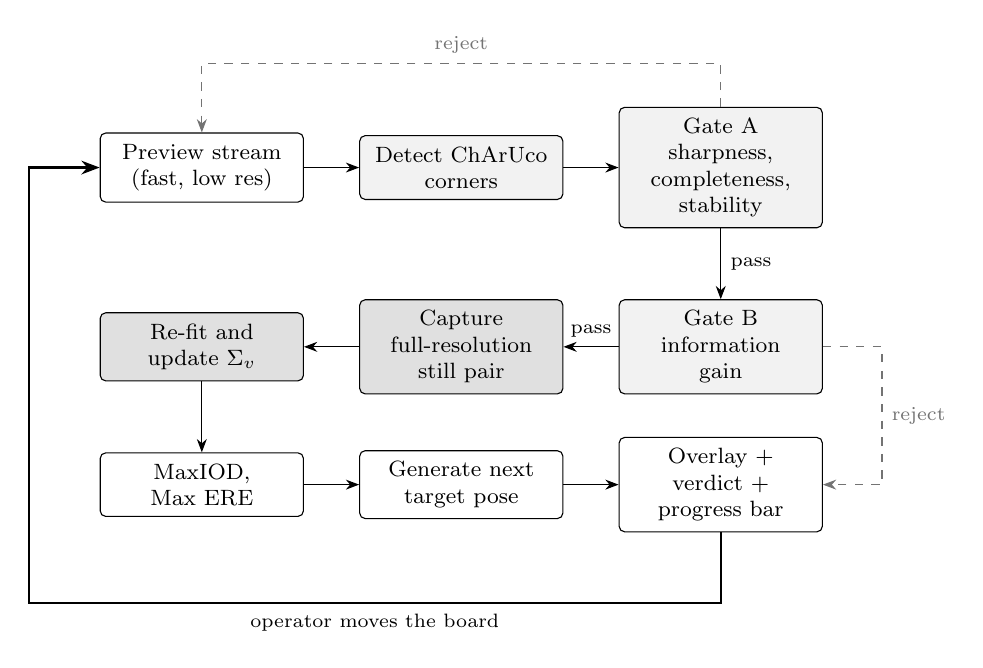
\begin{tikzpicture}[
  font=\footnotesize,
  box/.style={draw, rounded corners=2pt, align=center, inner sep=4pt, minimum height=8mm, text width=23mm},
  gate/.style={box, fill=black!5},
  keep/.style={box, fill=black!12},
  >=Stealth, node distance=5mm]

\node[box] (prev) {Preview stream\\(fast, low res)};
\node[gate, right=7mm of prev] (det) {Detect ChArUco\\corners};
\node[gate, right=7mm of det] (gate1) {Gate A\\sharpness,\\completeness,\\stability};
\node[gate, below=9mm of gate1] (gate2) {Gate B\\information\\gain};
\node[keep, left=7mm of gate2] (still) {Capture\\full-resolution\\still pair};
\node[keep, left=7mm of still] (fit) {Re-fit and\\update $\Sigma_v$};

\node[box, below=9mm of fit] (metric) {MaxIOD,\\Max ERE};
\node[box, right=7mm of metric] (pose) {Generate next\\target pose};
\node[box, right=7mm of pose] (ui) {Overlay +\\verdict +\\progress bar};

\draw[->] (prev) -- (det);
\draw[->] (det) -- (gate1);
\draw[->] (gate1) -- node[right, font=\scriptsize] {pass} (gate2);
\draw[->] (gate2) -- node[above, font=\scriptsize] {pass} (still);
\draw[->] (still) -- (fit);
\draw[->] (fit) -- (metric);
\draw[->] (metric) -- (pose);
\draw[->] (pose) -- (ui);

% reject paths
\draw[->, dashed, black!55] (gate1.north) -- ++(0,0.55) -| node[pos=0.25, above, font=\scriptsize] {reject} (prev.north);
\draw[->, dashed, black!55] (gate2.east) -- ++(0.75,0) |- node[pos=0.25, right, font=\scriptsize] {reject} (ui.east);

% feedback to operator: routed around the left of the column so it crosses nothing
\coordinate (farleft) at ([xshift=-9mm]prev.west);
\coordinate (d1) at ([yshift=-9mm]ui.south);
\coordinate (d2) at (farleft |- d1);
\draw[->, thick] (ui.south) -- (d1)
      -- node[below, font=\scriptsize, pos=0.5] {operator moves the board} (d2)
      -- (farleft) -- (prev.west);

\end{tikzpicture}
\caption[Architecture of the proposed calibration loop]{The proposed loop. The preview stream drives detection and guidance at interactive rates; only frames that pass both gates trigger a full-resolution capture. Everything below the dashed rejection paths runs once per accepted frame, not once per preview frame.}
\label{fig:loop}
\end{figure}

\section{Video or stills? Both, for different jobs}

The instinct to replace discrete photographs with a continuous stream is right, but a calibration cannot simply be run on a video, for a reason established in Section \ref{sec:resolution}: on this sensor the video modes are not the still mode. The 2028$\times$1080 and 1332$\times$990 modes are cropped as well as binned, so a calibration computed from them describes a different optical configuration than the 4056$\times$3040 captures the experiment will use (Table \ref{tab:modes}).

The resolution is to use each stream for what it is good at:

\begin{itemize}
    \item \textbf{The preview stream drives interaction.} Detection, pose estimation, the live verdict and the guidance overlay all run on the low-resolution stream, which is fast enough to feel continuous. Nothing from this stream enters the calibration.
    \item \textbf{Accepted poses trigger a full-resolution still pair.} Only frames that pass both gates cause a capture at 4056$\times$3040 with an explicit sensor mode. These are the only images that are fitted.
\end{itemize}

This keeps the operator experience continuous while guaranteeing that every image in the solution came from the mode the calibration will be used in. It also matches how the reviewed systems behave in practice: the operator is guided towards a pose and the image is taken when the pose is reached \cite{peng2019wizard,rojtberg2018pose}.

\section{Gate A: is this frame usable at all?}

Gate A rejects frames that are bad regardless of where the board is. It runs on every preview frame.

\begin{table}[!ht]
\centering
\small
\caption[Gate A criteria]{Per-frame rejection criteria. These are cheap and run continuously.}
\label{tab:gatea}
\begin{tabularx}{\textwidth}{p{0.17\textwidth} p{0.30\textwidth} X}
\toprule
\textbf{Check} & \textbf{Test} & \textbf{Why} \\
\midrule
Completeness & Number of detected ChArUco corners above a floor & Too few points makes the per-view pose ill-conditioned. ChArUco tolerates partial views, which is why it is used \cite{garrido2014aruco,rojtberg2018pose} \\
Sharpness & Focus measure over the detected board region, not the whole frame & A board outside the depth of field degrades corner localisation. This is the suspected cause of the previous failures (Section \ref{sec:hypothesis}) \\
Stability & Corner displacement between consecutive preview frames below a threshold & Rejects motion blur and ensures the full-resolution capture that follows sees the same pose \\
Exposure & No saturated or crushed regions on the board & Clipped corners localise poorly \\
\bottomrule
\end{tabularx}
\end{table}

The sharpness check deserves emphasis. It is the cheapest single addition that addresses the hypothesis of Section \ref{sec:hypothesis}, and it is the one the current procedure most clearly lacks: at f/1.6 the usable depth is about one metre, and nothing in the present workflow warns the operator when the board leaves it.

\section{Gate B: would this frame improve the calibration?}

Gate A asks whether the image is good. Gate B asks the harder question, whether it is \emph{useful}. This is where the user's concern about frames that worsen the result is addressed.

A frame can be perfectly sharp, fully detected and still worthless, because it duplicates a pose already captured. Worse, a set dominated by near-parallel views is actively misleading: it produces a low residual while leaving the focal length unconstrained (Section \ref{sec:degeneracy}).

Gate B is therefore an information-gain test against the current state:

\begin{enumerate}
    \item Estimate the board pose from the preview detection.
    \item Check it against the non-degeneracy rules of Section \ref{sec:degeneracy}: not parallel to the image plane, not parallel to either image axis, and not violating the reflection constraint with respect to the poses already held \cite{rojtberg2018pose}.
    \item Check that it advances the currently targeted parameter, which is the one with the largest index of dispersion, the MaxIOD of Equation \ref{eq:iod}.
    \item Accept only if it does both.
\end{enumerate}

Two implementation notes. First, the strict version of step 3 predicts the covariance that would result from adding this frame, which requires one extra Jacobian evaluation; the cheap version compares the pose against the target pose the tool is currently suggesting and accepts when it is close enough. The reviewed systems use the cheap version at interaction time \cite{peng2019wizard,rojtberg2018pose}. Second, a frame that is rejected by Gate B is not an error, and the interface should say so differently from a Gate A rejection: the board is fine, it is in the wrong place.

\section{The verdict and the progress bar}

\subsection{Per-frame verdict}

The operator should see, on every preview frame, one of four states: \emph{board not found}, \emph{rejected and why} (blurred, moving, clipped, too few corners), \emph{good board but wrong pose, move here}, or \emph{captured}. The third state is the one that teaches, and it should be accompanied by the overlay of the suggested next pose, which is the mechanism Rojtberg's user study found sufficient to bring novices to a precise calibration in roughly two minutes \cite{rojtberg2019guidance}.

\subsection{What the progress bar should actually show}

A bar driven by a frame count is misleading, because it implies that the twentieth image is worth as much as the second. The bar should be driven by the convergence state of the parameters.

Two complementary displays are proposed:

\begin{itemize}
    \item \textbf{Per-parameter bars}, one for each of the nine intrinsics plus the stereo transform, showing the index of dispersion of Equation \ref{eq:iod} against its convergence threshold. This tells the operator \emph{which} parameter is currently holding the session back, which is exactly the parameter the suggested pose is targeting. The authors report that this covariance correlates with testing error \cite{rojtberg2018pose}.
    \item \textbf{A single overall figure in pixels}, the Max ERE of Section \ref{chap:quality}, shown against the accuracy budget. This is the number that answers ``is it good enough yet'' in units the operator can reason about \cite{richardson2013aprilcal}.
\end{itemize}

The session ends when all parameters pass the ratio test of Equation \ref{eq:ratio} and Max ERE is below budget, which is criteria C1 and C2 of Table \ref{tab:acceptance}. It does not end at a fixed image count.

\section{The stereo extension}

Everything above is per-camera. For the LINKU rig the inter-camera transform $R, T$ must also be constrained, and a pose that is informative for one camera's intrinsics is not automatically informative for the stereo pair. Two additions follow from Tan et al. \cite{tan2025stereoposes}:

\begin{itemize}
    \item Gate A gains a binocular condition: the board must be fully detected in \emph{both} cameras simultaneously for the frame to contribute to the stereo extrinsics.
    \item The convergence state extends to cover $R$ and $T$, using the trace of the covariance as the scalar objective, with the relative and absolute extrinsics optimised jointly rather than separately.
\end{itemize}

Because the two cameras are rigidly coupled at a 100~mm baseline, the region where both see the board at a useful angle is smaller than either camera's field. The guidance must propose poses inside that intersection, otherwise it will repeatedly suggest poses that one camera cannot see.

\section{What the tool must preserve from the current code}

Three behaviours in the existing implementation are correct and must survive the rewrite:

\begin{enumerate}
    \item Calibration captures are forced to \texttt{capture\_resolution} with an explicit \texttt{-{}-mode}, so the sensor mode is not chosen silently (Section \ref{sec:resolution}).
    \item Both cameras are captured as a synchronised pair with the time difference recorded in the session metadata.
    \item Each session is written to its own timestamped directory with per-pair metadata, which is what makes the retrospective analysis of Section \ref{sec:hypothesis} possible at all.
\end{enumerate}

\section{What this does not solve}

The tool improves the \emph{procedure}. It does not compensate for a lens whose focus ring has moved since the session, for a board that is not flat, or for a calibration applied at a different sensor mode. Those remain operational disciplines, and they are the content of Table \ref{tab:failures}. The tool can, however, detect the second of them after the fact, through the bias ratio of Section \ref{chap:quality}.

\chapter{Implementation Plan Against the Existing Code}
\label{chap:plan}

The proposal of Chapter \ref{chap:design} is not a rewrite. A survey of the current implementation shows that roughly half of the required machinery is already present and in the right place; what is missing is the feedback loop that connects it.

\section{What already exists}

\begin{table}[!ht]
\centering
\small
\caption[Existing calibration code relevant to the proposal]{Components already present in \texttt{camera/camera\_calibration.py}, and how the proposal uses them.}
\label{tab:existing}
\footnotesize
\setlength{\tabcolsep}{4pt}
\begin{tabularx}{\textwidth}{>{\raggedright\arraybackslash}p{0.30\textwidth} p{0.13\textwidth} X}
\toprule
\textbf{Existing component} & \textbf{Status} & \textbf{Role in the proposal} \\
\midrule
\texttt{detect\_charuco\_corners} & Ready & Gate A detection. ChArUco is already the chosen target, matching \cite{rojtberg2018pose} \\
\texttt{\_process\_charuco\_\allowbreak calibration} & Ready & The fit \\
\texttt{execute\_stereo\_\allowbreak calibration\_charuco} & Ready & Stereo extrinsics \\
\texttt{validate\_image\_quality} & \textbf{Needs work} & Already computes sharpness, contrast, coverage, board angle and illumination uniformity. But it runs after the session, not live, and two of its details are wrong (below) \\
\texttt{validate\_calibration\_\allowbreak quality} & \textbf{Needs replacing} & Decides \texttt{is\_good\_quality} from the reprojection error alone, the metric Chapter \ref{chap:quality} rules out \\
Session directories with per-pair metadata & Ready & Enables the retrospective study of Section \ref{sec:hypothesis} \\
Explicit \texttt{-{}-mode} on calibration captures & Ready & Guarantees the sensor mode matches (Section \ref{sec:resolution}). Must be preserved \\
\bottomrule
\end{tabularx}
\end{table}

\subsection{Two defects in the existing quality check}

\textbf{The sharpness measure is computed over the whole frame.} \texttt{validate\_image\_quality} takes the variance of the Laplacian over the entire image. In a dark room with a black background, most of the frame is empty, so the measure is dominated by the background and is largely insensitive to whether the \emph{board} is in focus. It should be computed over the bounding region of the detected corners, which the function already has available as an argument.

\textbf{The sharpness threshold appears far too permissive.} The current rejection threshold is a Laplacian variance of 3.0. Values that low correspond to an almost featureless image; a sharply imaged chessboard typically produces values orders of magnitude higher. As written, the check will pass nearly every frame, including badly defocused ones. This is consistent with the hypothesis of Section \ref{sec:hypothesis} and should be recalibrated empirically against the archived sessions rather than guessed.

\section{Staged plan}

The stages are ordered so that each delivers something usable on its own, and so that the cheapest diagnostic comes first.

\begin{table}[!ht]
\centering
\small
\caption[Staged implementation plan]{Proposed stages. Effort is indicative and assumes work against the existing codebase.}
\label{tab:stages}
\begin{tabularx}{\textwidth}{p{0.04\textwidth} p{0.26\textwidth} X p{0.09\textwidth}}
\toprule
\textbf{\#} & \textbf{Stage} & \textbf{Content} & \textbf{Effort} \\
\midrule
S0 & Retrospective diagnosis & \textbf{Done.} Gate A and Gate B measures run over the whole archive; result in Section \ref{sec:hypothesis}. Delivered as \texttt{camera/calibration\_guidance.py} and \texttt{tools/\allowbreak analyze\_calibration\_sessions.py} & 4 h \\
S1 & Live Gate A & \textbf{Logic done, not wired.} The corrected measures and the per-frame verdict exist in \texttt{evaluate\_frame}; what remains is to call them from the preview loop of \texttt{gui/\allowbreak calibration\_dialog.py} and draw the result & 4 h left \\
S2 & Honest metrics & \textbf{Done.} Parameter covariance via OpenCV's \texttt{stdDeviations\allowbreak Intrinsics}, index of dispersion, ratio-test convergence and an approximate Max ERE \cite{richardson2013aprilcal,rojtberg2018pose}. \texttt{validate\_calibration\_quality} still needs replacing in the old path & 2 h left \\
S3 & Progress indicator & \textbf{Computed, not drawn.} \texttt{SessionStatus} reports coverage, convergence and an overall figure; the bars and the Max ERE readout are not yet in the interface & 4 h left \\
S4 & Gate B and pose guidance & \textbf{Partial.} The non-degeneracy rules, the duplicate-pose test and tilt-bin coverage are implemented and enforced. The analytic pose generator of \cite{rojtberg2018pose}, binary subdivision of the tilt range with the 22.5\textdegree{} rotation and the distortion map, and the on-screen overlay of the target pose, are not & 12 h left \\
S5 & Stereo extension & Binocular gating and the joint extrinsic criterion \cite{tan2025stereoposes} & 10 h \\
S6 & Post-session audit & Bias ratio and Expected Mapping Error as an offline report \cite{hagemann2021bias} & 8 h \\
\bottomrule
\end{tabularx}
\end{table}

\subsection{S0 has been run, and it reprioritised the rest}

Stage S0 was the one stage that could be executed immediately, and it was. The reasoning for running it first was that the archive could show either of two things: inadequate sharpness, in which case S1 alone might suffice, or adequate sharpness with no angular spread, in which case the problem is degeneracy and S4 becomes the priority.

The measurement, reported in Section \ref{sec:hypothesis}, gave the second answer unambiguously. Sharpness over the board is adequate and detection succeeds; the board was simply never tilted. The consequence for this table is that \textbf{S4 is the stage that addresses the cause}, and S1, while still worth having, no longer sits on the critical path.

\subsection{What exists today}

Four files have been written, none of which depends on a camera or on the interface, so all of them can be exercised offline against the archive.

\begin{itemize}
    \item \texttt{camera/calibration\_guidance.py}: the measures. Gate A frame quality, the degeneracy and novelty tests of Gate B, parameter uncertainty and the index of dispersion, the convergence ratio test, and an approximate Max ERE.
    \item \texttt{camera/guided\_session.py}: the loop. Frames are offered continuously; a rejected frame does not consume one of the requested slots, so asking for 25 views yields 25 views that passed both gates. The session refuses to report itself complete until the accepted set covers the tilt bins of Table \ref{tab:bins}.
    \item \texttt{tools/analyze\_calibration\_sessions.py}: the retrospective diagnosis of Section \ref{sec:hypothesis}.
    \item \texttt{tools/replay\_guided\_session.py}: replays an archived session through the loop one frame at a time, which is how the loop is tested without hardware.
\end{itemize}

\begin{table}[!ht]
\centering
\small
\caption[Tilt bins the accepted set must cover]{Pose-space coverage enforced by the session. The frontal bin serves the distortion coefficients, which need frontal views at the image edges; the tilted bins serve the pinhole parameters, which need angular spread \cite{rojtberg2018pose}. Three views per bin is the shipped default.}
\label{tab:bins}
\begin{tabular}{lll}
\toprule
\textbf{Bin} & \textbf{Tilt} & \textbf{Serves} \\
\midrule
frontal          & 0--10\textdegree  & distortion terms \\
slightly tilted  & 15--30\textdegree & pinhole \\
clearly tilted   & 30--45\textdegree & pinhole \\
strongly tilted  & 45--70\textdegree & pinhole \\
\bottomrule
\end{tabular}
\end{table}

\subsection{What the loop does on the archived sessions}

Replaying the three February 2026 sessions through the loop is the validation that it behaves as intended, and it reproduces the diagnosis independently. Results in Table \ref{tab:replay}.

\begin{table}[!ht]
\centering
\small
\caption[Archived sessions replayed through the guided loop]{Each archived session replayed frame by frame. Every one is refused completion, and for the same reason: no session contains a single view above 45\textdegree{} of tilt.}
\label{tab:replay}
\begin{tabularx}{\textwidth}{l c c c X}
\toprule
\textbf{Session} & \textbf{Offered} & \textbf{Kept} & \textbf{Spread} & \textbf{Verdict} \\
\midrule
\texttt{...\_152124} & 25 & 3  & 1.1\textdegree  & Only the frontal bin filled; 18 frames refused as duplicate poses \\
\texttt{...\_155926} & 25 & 12 & 41.0\textdegree & Three bins filled, 45--70\textdegree{} empty \\
\texttt{...\_160735} & 20 & 9  & 29.4\textdegree & Three bins filled, 45--70\textdegree{} empty \\
\bottomrule
\end{tabularx}
\end{table}

The first row is the clearest demonstration of the contract. Twenty-five frames were offered and three were kept, because the other twenty-two carried no information the first three had not already supplied. A procedure that counts photographs would have recorded that session as complete. The module carries no camera or interface dependency, so stages S1 to S5 can be built on top of it without rework.

\subsection{A note on reusing published code}

Rojtberg and Kuijper's method is published with a working implementation, \texttt{pose\_calib}, built on OpenCV and the same ChArUco functions this project already calls \cite{rojtberg2018pose}. Calibration Wizard is likewise published with demo code \cite{peng2019wizard}. Stages S2 and S4 should begin by reading those implementations rather than deriving the algorithms afresh. Neither is a drop-in dependency, because both are monocular and this project needs the stereo case, but the covariance and pose-generation logic transfers directly.

\section{Interaction with the rest of the project}

\begin{itemize}
    \item \textbf{Illumination.} The calibration session must be lit well enough for the board to be sharp and unclipped. The requirements, and the depth-of-field figures used in Section \ref{sec:hypothesis}, are in the companion deliverable \cite{linku_darkroom_illumination}.
    \item \textbf{Optical discipline.} The focus and aperture rings must be set and locked before the session, and not touched afterwards, for the reasons in Chapter \ref{chap:failure}. The companion deliverable specifies the locking and marking procedure.
    \item \textbf{Geometry.} The calibration must be performed on the integrated camera support that will be used in the experiment, not on a different mount. Moving the cameras between calibration and use invalidates the stereo extrinsics.
\end{itemize}

\todo[inline]{Next: before building anything further, repeat one calibration session with the board deliberately tilted between roughly 20 and 60 degrees and at full sensor resolution. Section \ref{sec:hypothesis} shows that is the single change most likely to produce a usable calibration, and it needs no new software. Re-run \texttt{tools/analyze\_calibration\_sessions.py} on the result to confirm the angular spread before fitting.}

\chapter{Conclusion}

\section{Direct answers to the questions asked}

\begin{table}[!ht]
\centering
\small
\caption[Answers to the operator questions]{The questions that prompted this document, and where each is answered.}
\label{tab:answers}
\begin{tabularx}{\textwidth}{p{0.29\textwidth} X p{0.10\textwidth}}
\toprule
\textbf{Question} & \textbf{Answer} & \textbf{Section} \\
\midrule
Do intrinsics and extrinsics come from different photographs? & No. Both are solved jointly from the same images. Tilting the board is what makes the \emph{intrinsics} observable & \ref{chap:failure}.1 \\
Must all images share one resolution? & Yes, and the same sensor mode. Two of the IMX477 modes are cropped as well as binned, so a calibration cannot be rescaled into them & \ref{sec:resolution} \\
Does moving the focus break the calibration? & Yes. It changes the focal length and therefore biases the scale of every reconstructed distance & \ref{chap:failure}.3 \\
Does moving the aperture break it? & Much less. It shifts the principal point and distortion slightly, but it is not geometrically catastrophic. Calibrate at the working aperture & \ref{chap:failure}.4 \\
Could capture be continuous, like video? & Yes for the interaction, no for the images. Guide on the preview stream, capture accepted poses as full-resolution stills & \ref{chap:design}.2 \\
How do we filter frames that do not help? & Two gates: one for image quality, one for information gain against the current parameter uncertainty & \ref{chap:design}.3--4 \\
Can we show a progress bar? & Yes, and it should be driven by parameter uncertainty and Max ERE, not by an image count & \ref{chap:design}.5 \\
\bottomrule
\end{tabularx}
\end{table}

\section{The central finding}

Every failure mode catalogued in Table \ref{tab:failures} shares one property: more images do not fix it. A calibration session that is degenerate, defocused or captured in the wrong sensor mode will not converge no matter how long it runs, and the metric currently used to judge the result, the root-mean-square reprojection error, is structurally incapable of revealing any of them because it measures how well the model fits the data it was trained on.

That is why the proposal is a feedback loop rather than a better checklist. The published systems all reach the same architecture independently \cite{richardson2013aprilcal,rojtberg2018pose,peng2019wizard,tan2025stereoposes}: estimate the covariance of the parameters while the session runs, use it to decide where the board should go next, and use it again to decide when to stop. With that loop in place, Rojtberg reports novice users completing a precise calibration in about two minutes \cite{rojtberg2019guidance}.

\section{What should happen next}

Stage S0 of Table \ref{tab:stages} has been run, and it settled the question: the failures are geometric, not optical. The board was held nearly flat in 91\% of the archived frames, which makes the focal length unrecoverable regardless of how many images are taken (Section \ref{sec:hypothesis}).

That outcome reprioritises the plan. \textbf{Stage S4, pose guidance, is now the stage that fixes the actual problem}, and S1, the live quality gate, drops from prerequisite to useful hygiene. The fastest route to a usable calibration is in fact neither: it is to repeat a session with the board deliberately tilted across a wide angular range, between roughly 20 and 60 degrees, which costs one session and requires no software at all. S4 then makes that outcome repeatable rather than dependent on the operator remembering to tilt.

\section{Confidence and limitations}

\begin{table}[!ht]
\centering
\small
\caption[Status of the claims in this document]{Where each part of the argument stands.}
\label{tab:confidence}
\begin{tabularx}{\textwidth}{p{0.30\textwidth} p{0.12\textwidth} X}
\toprule
\textbf{Claim} & \textbf{Status} & \textbf{Basis} \\
\midrule
Reprojection error is not a quality metric & Firm & Stated independently in \cite{rojtberg2018pose,richardson2013aprilcal,hagemann2021bias} \\
Parallel-only views make the focal length unrecoverable & Firm & Derived in \cite{rojtberg2018pose} from the projection equations \\
Resolution and sensor mode must match & Firm & Follows from Equation \ref{eq:fx}; mode table computed from published Raspberry Pi specifications \\
Focus drift biases reconstruction scale & Firm & Direct consequence of Equation \ref{eq:fx} \\
Aperture has a smaller geometric effect & Reasoned & Standard optical argument; no source in the reviewed set quantifies it for this lens class \\
Degeneracy caused the failures & \textbf{Measured} & Stage S0 was run over the archive. Median board tilt 4.4\textdegree, no frame above 45\textdegree, 91\% of poses degenerate, and $f_x$ uncertain by 0.85\% at an RMS of 1.50~px (Sec. \ref{sec:hypothesis}) \\
Defocus caused the failures & \textbf{Refuted} & The hypothesis of an earlier draft of this document. Sharpness over the board region is adequate and detection succeeds; the problem is geometric, not optical \\
The proposed design will work here & Projected & Each component is published and validated elsewhere; the combination, and the stereo case specifically, has not been built for this rig \\
Effort estimates in Table \ref{tab:stages} & Indicative & Not derived from measurement \\
\bottomrule
\end{tabularx}
\end{table}

The most important line in that table is the sixth. The explanation offered for the 23 failed attempts is a well-supported hypothesis, not a finding, and this document should not be read as having diagnosed the problem. It has identified the most likely cause and specified the half-day experiment that would confirm it.


\bibliographystyle{ieeetr}
\bibliography{bibs/sample}

\end{document}
